\section{Estudio de la API de Spotify}

La API de Spotify es el núcleo del proyecto, ya que proporciona acceso a los datos necesarios para generar las estadísticas y visualizaciones que constituyen el objetivo principal de este trabajo. Este capítulo detalla el análisis realizado sobre la API, explorando sus capacidades, limitaciones y los recursos que ofrece para su integración.

\subsection{Descripción General}

La API de Spotify es una interfaz que permite a las aplicaciones externas interactuar con la plataforma de manera programática. Su propósito principal es proporcionar acceso estructurado a los datos, permitiendo a los desarrolladores integrar funcionalidades avanzadas en sus propias aplicaciones. A través de esta API, es posible obtener información sobre las canciones, artistas, álbumes, listas de reproducción y \textbf{datos personalizados del usuario}, como sus preferencias musicales o sus hábitos de escucha. Gracias a estos últimos, es posible ofrecer una experiencia personalizada para cada usuario.

Entre las características técnicas más destacadas se encuentran:

\begin{itemize}
    \item \textbf{Tipo de API}: RESTful.
    \item \textbf{Protocolo}: HTTPS.
    \item \textbf{Métodos soportados}: \texttt{GET}, \texttt{POST}, \texttt{PUT} y \texttt{DELETE}.
    \item \textbf{Formato de respuesta}: JSON
    \item \textbf{Seguridad}: Acceso protegido mediante OAuth 2.0.
\end{itemize}

Gracias a estas características, la API de Spotify facilita la manipulación de datos gracias a las respuestas en formato JSON, al tiempo que garantiza la seguridad y privacidad del usuario mediante el uso del protocolo OAuth 2.0. Estas cualidades la convierten en una herramienta versátil y segura, capaz de adaptarse a una amplia variedad de proyectos.

\subsection{Autenticación y Autorización}

Antes de avanzar, es importante entender que en este proceso hay dos conceptos clave: \textbf{autenticación} y \textbf{autorización}. Aunque están relacionados, existen ciertas diferencias importantes:

\begin{itemize}
    \item \textbf{Autenticación}: Es el paso en el que se \underline{verifica la identidad} del usuario. En este caso, ocurre cuando el usuario inicia sesión en Spotify para confirmar que es quien dice ser. Este proceso es transparente para el desarrollador ya que Spotify, mediante OAuth 2.0, se encarga de gestionarlo.
    \item \textbf{Autorización}: Es el paso en el que el usuario \underline{concede permisos} para que la aplicación acceda a ciertos recursos de su cuenta. Este proceso es clave, ya que sin estos permisos, la aplicación no podría acceder a los datos necesarios para ofrecer sus funcionalidades.
\end{itemize}

Una vez que la aplicación obtiene la autorización, Spotify permite el acceso a los datos solicitados de forma controlada. Un concepto fundamental en esta etapa son los \textbf{scopes}, que determinan exactamente qué datos y funcionalidades están disponibles para la aplicación.

\subsubsection*{Scopes: Controlando el Acceso a los Recursos}

Los scopes (alcances) permiten a los usuarios tener la tranquilidad de que únicamente compartirán la información que han autorizado explícitamente. Cuando un programador configura el flujo de autorización, debe especificar los scopes necesarios (de un total de 24) para que la aplicación pueda acceder a los recursos protegidos. En función de los scopes solicitados, Spotify mostrará al usuario una pantalla indicando qué permisos específicos se están requiriendo (figura \ref{fig:auth_popup}). El usuario puede entonces aceptar o rechazar estos permisos.

\begin{figure}[H]
    \centering
    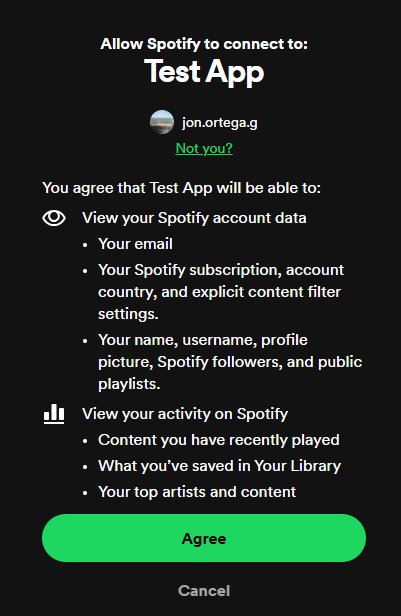
\includegraphics[width=0.3\textwidth]{./figures/auth_popup.png}
    \caption{Pantalla de autorización de scopes en Spotify.}
    \label{fig:auth_popup}
\end{figure}

Una vez que la aplicación obtiene la autorización, el siguiente paso es conseguir el \texttt{access\_token}, necesario para acceder a los recursos autorizados. Un concepto clave para entender cómo se realiza este proceso es el \textbf{authorization flow}, que define las interacciones entre la aplicación, el usuario y Spotify.

\subsubsection*{OAuth Flows: Elegir el Camino Adecuado}

En el marco de OAuth 2.0, el término \textbf{flow} (flujo) se refiere a los diferentes procesos diseñados para obtener un \texttt{access\_token}, dependiendo de las necesidades y características de la aplicación. Estos flujos existen para cubrir una variedad de escenarios, desde aplicaciones web con servidores backend hasta aplicaciones móviles o servicios que no requieren acceso a datos del usuario.

OAuth 2.0 define seis tipos principales de flows, sin embargo, Spotify implementa solo cuatro de ellos (tabla \ref{tab:oauth_spotify_flows}):

\begin{table}[H]
    \centering
    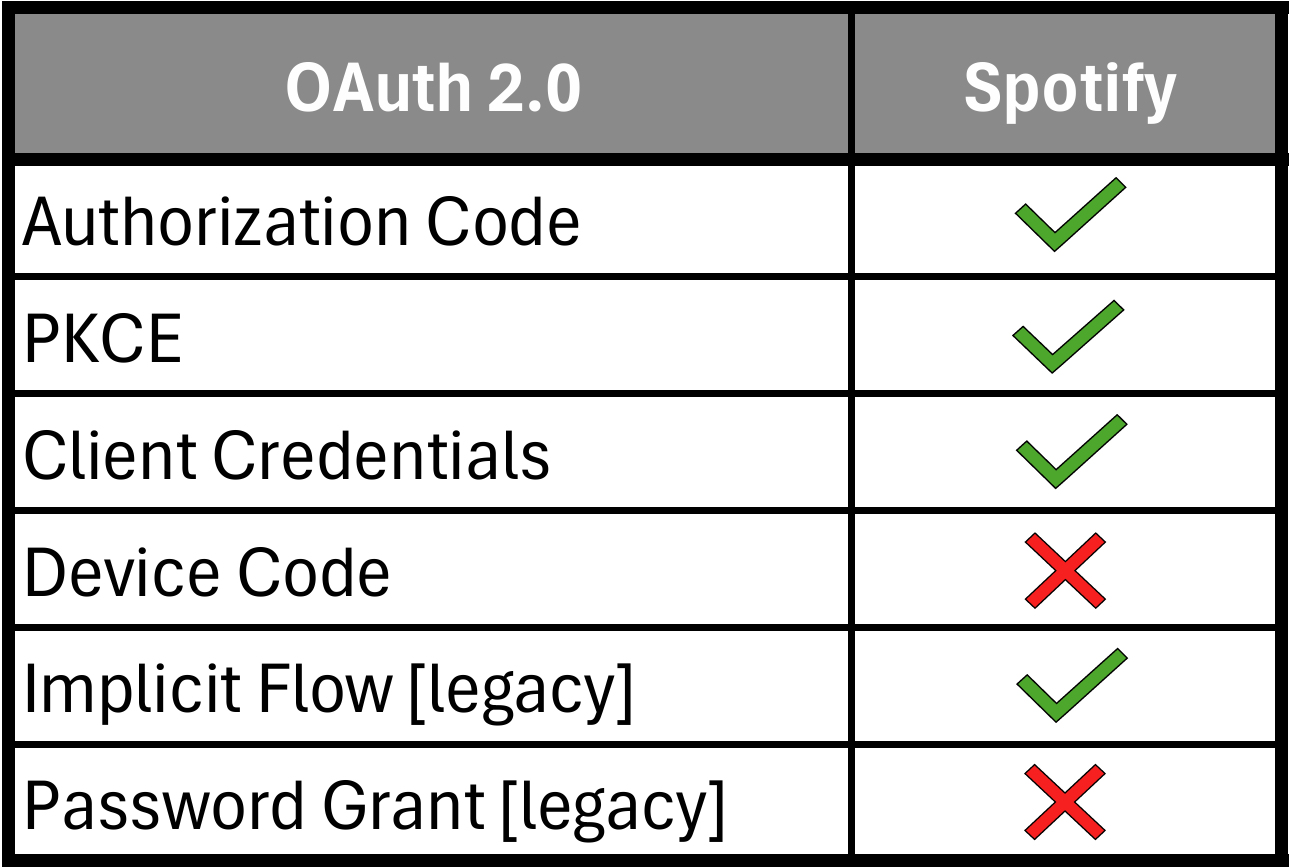
\includegraphics[width=0.5\textwidth]{figures/oauth_vs_spotify_flows.png}
    \caption{Authorization flows definidos por OAuth 2.0 y cuáles implementa Spotify.}
    \label{tab:oauth_spotify_flows}
\end{table}

Cada uno de estos flujos está diseñado para un escenario específico de uso, por lo que, para poder tomar una buena elección, analizaremos las situaciones en las que cada uno resulta más adecuado:

\begin{itemize}
    \item \textbf{Authorization Code Flow}: Ideal para aplicaciones web que cuentan \underline{con un backend} \underline{seguro} donde almacenar el \texttt{client\_secret}. Proporciona tanto un \texttt{access\_token} como un \texttt{refresh\_token}, lo que permite mantener el acceso sin requerir que el usuario se autentique nuevamente. Es el flujo recomendado para aplicaciones con servidores backend que necesitan acceso a datos específicos del usuario.

    \item \textbf{Authorization Code Flow con PKCE}: Es una extensión del anterior, diseñado para \underline{escenarios donde no es seguro almacenar el \texttt{client\_secret}}, como en aplicaciones móviles o \textit{Single Page Applications} (SPA). Añade una capa de seguridad utilizando un \texttt{code\_verifier} y un \texttt{code\_challenge} para evitar que el código de autorización sea interceptado y utilizado de manera malintencionada.

    \item \textbf{Client Credentials Flow}: Adecuado para aplicaciones backend o \underline{servicios que no} \underline{requieren acceso a datos específicos del usuario}, sino que interactúan con recursos de Spotify de manera general. No incluye un proceso de autorización por parte del usuario y no proporciona datos personales.

    \item \textbf{Implicit Grant Flow}: \underline{En desuso debido a limitaciones de seguridad}. Fue diseñado para aplicaciones cliente que no tienen un backend, pero carece de soporte para \texttt{refresh\_tokens} y expone el \texttt{access\_token} en la URL, lo que lo hace menos seguro.
\end{itemize}

De los cuatro flujos de autorización implementados por Spotify, este proyecto utilizará el \textbf{Authorization Code Flow} (sin PKCE). Esta elección se debe a que la aplicación cuenta con un backend seguro implementado con API Routes de Next.js, lo que permite almacenar de forma segura el \texttt{client\_secret}. Además, este flujo proporciona tanto un \texttt{access\_token} como un \texttt{refresh\_token}, lo que asegura un acceso continuo a los datos del usuario sin necesidad de repetir el proceso de autenticación. Dado que es el flujo recomendado por Spotify para aplicaciones web que necesitan acceder a datos específicos del usuario, garantiza un balance óptimo entre seguridad, funcionalidad y cumplimiento de estándares.

\subsection{Principales Endpoints Relevantes para el Proyecto}

Para facilitar la comprensión de los endpoints utilizados en este proyecto, se ha diseñado un sistema visual que resume la información clave de cada uno, evitando la sobrecarga de texto y permitiendo al lector identificar rápidamente los elementos esenciales.

Cada endpoint se presenta como una interacción entre la solicitud (\textit{request}) y la respuesta (\textit{response}). A la izquierda, la \textit{request} incluye el método HTTP (\texttt{GET}, \texttt{POST}, \texttt{PUT}, \texttt{DELETE}), la URL de la petición y los parámetros requeridos, que pueden estar en la URL (para métodos \texttt{GET}) o en el cuerpo de la solicitud (\textit{body}, para métodos como \texttt{POST} o \texttt{PUT}). Si existen parámetros en los \textit{headers}, se mostrarán sobre los parámetros del \textit{body}/URL. A la derecha se encuentra la \textit{response}, con los campos principales que estarán presentes en el JSON devuelto por la API de Spotify, si la solicitud se procesa correctamente

En la figura \ref{fig:plantilla_endpoints} se muestra una plantilla genérica que sirve como referencia para entender este sistema visual, que se rellenará con la información específica de cada endpoint en las siguientes secciones.

\begin{figure}[H]
    \centering
    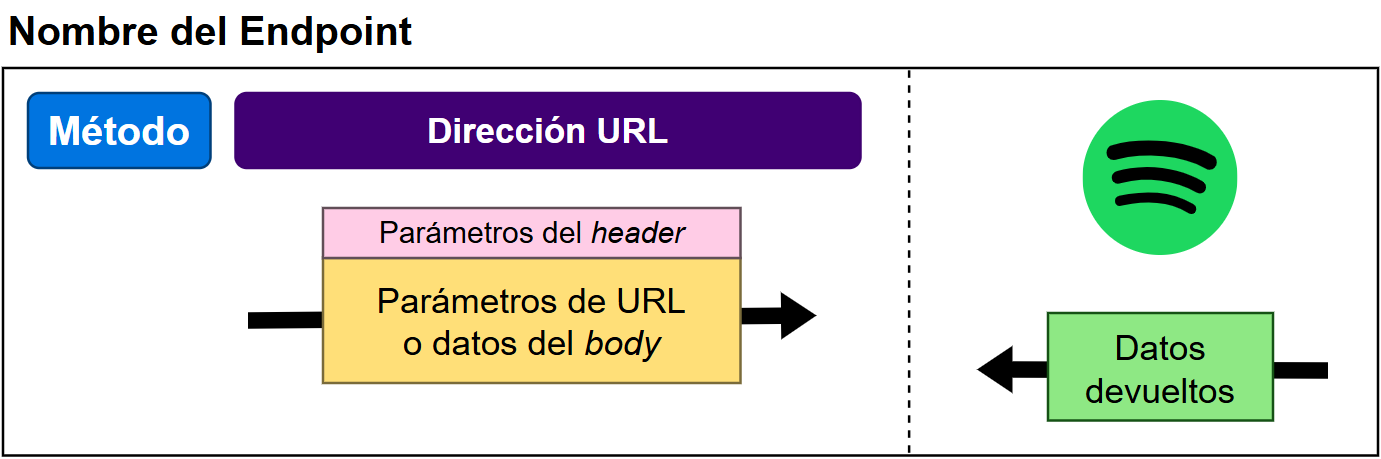
\includegraphics[width=0.95\textwidth]{figures/endpoints/plantilla_endpoints.png}
    \caption{Plantilla visual para representar los endpoints.}
    \label{fig:plantilla_endpoints}
\end{figure}

\subsubsection{Endpoints de Autenticación}

La interacción con Spotify comienza con un endpoint dedicado al proceso de autorización: \textbf{Request User Authorization} (figura \ref{fig:req_usr_auth}). Este endpoint genera la pantalla de autorización que se le muestra al usuario y, en el caso de que acepte, se le redirige a la \texttt{redirect\_uri} indicada en la \textit{request}. En esta URI siempre se suele implementar la llamada al segundo endpoint llamado \textbf{Request Access Token} (figura \ref{fig:req_access_token}), necesario para finalizar el proceso de autorización. Este permite intercambiar el \texttt{code} obtenido en el paso anterior por un \texttt{access\_token}, el cual es requerido para realizar cualquier otra solicitud posterior a la API.

\begin{figure}[H]
    \centering
    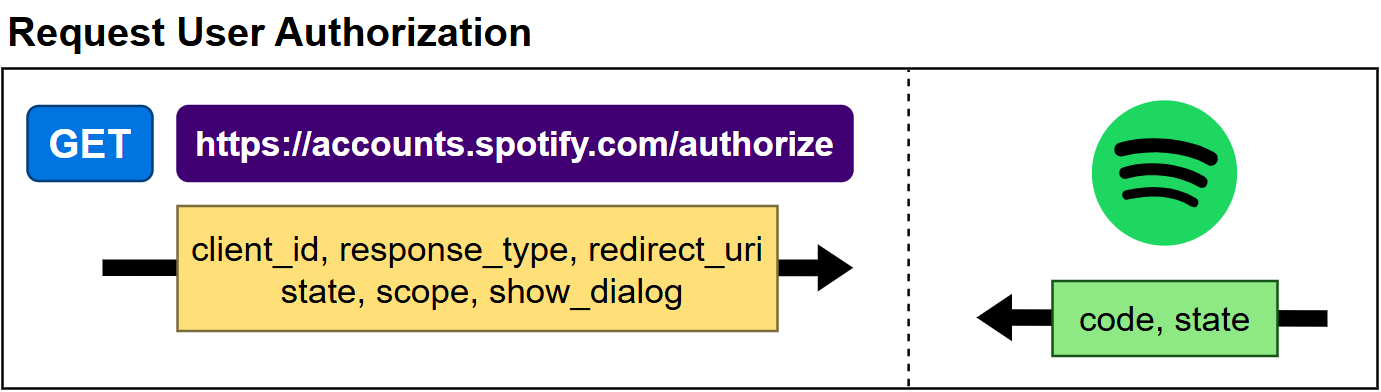
\includegraphics[width=\textwidth]{figures/endpoints/request_user_auth.png}
    \caption{Endpoint de \textit{Request User Authorization}.}
    \label{fig:req_usr_auth}
\end{figure}

\begin{itemize}
    \item \textbf{Parámetros del Request}
          \begin{itemize}
              \item \texttt{client\_id}: El ID de cliente generado al registrar la aplicación.
              \item \texttt{response\_type}: Se establece en \texttt{``code''}, indicando que se solicita un código de autorización.
              \item \texttt{redirect\_uri}: URI a la que se redirige al usuario después de aceptar o rechazar los permisos. Debe coincidir exactamente con uno de los valores configurados al registrar la aplicación.
              \item \texttt{state}: Parámetro utilizado para proteger contra ataques como \textit{cross-site request forgery} (CSRF). Su valor debe ser validado al recibir la respuesta.
              \item \texttt{scope}: Lista de scopes separados por espacios, indicando los permisos requeridos por la aplicación. Si no se especifican, solo se concederá acceso a información pública.
              \item \texttt{show\_dialog}: Determina si se fuerza al usuario a aprobar nuevamente la aplicación, incluso si ya lo hizo previamente. Si se establece en \texttt{true}, el usuario verá el diálogo de autorización; de lo contrario, será redirigido automáticamente.
          \end{itemize}
    \item \textbf{Parámetros del Response}
          \begin{itemize}
              \item \texttt{code}: Código de autorización que puede intercambiarse posteriormente por un \texttt{access\_token}.
              \item \texttt{state}: El valor del parámetro \texttt{state} enviado originalmente en la solicitud. Su valor debe ser comparado para garantizar la validez de la respuesta.
          \end{itemize}
\end{itemize}

\begin{figure}[H]
    \centering
    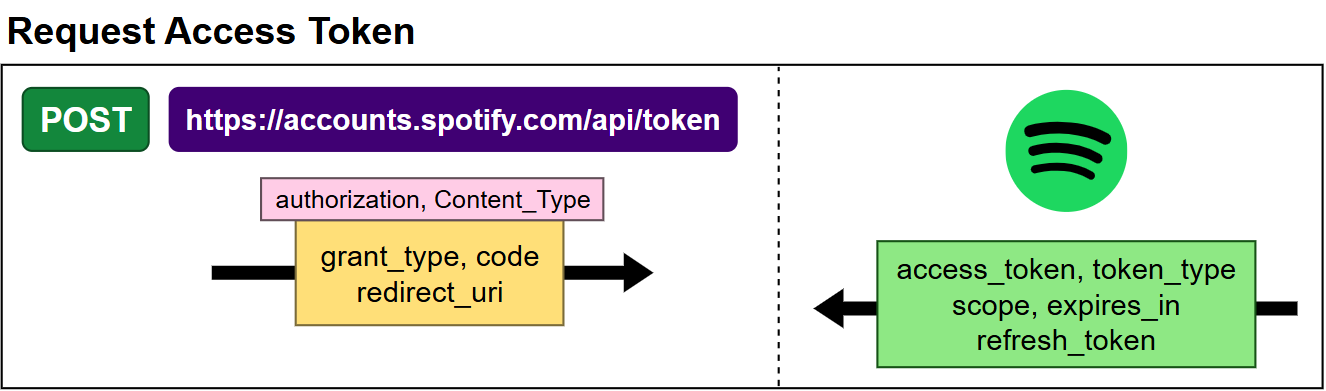
\includegraphics[width=\textwidth]{figures/endpoints/request_access_token.png}
    \caption{Endpoint de \textit{Request Access Token}.}
    \label{fig:req_access_token}
\end{figure}

\begin{itemize}
    \item \textbf{Parámetros del Request}
          \begin{itemize}
              \item \textbf{Body}
                    \begin{itemize}
                        \item \texttt{grant\_type}: Este campo debe contener el valor \texttt{``authorization\_code''}.
                        \item \texttt{code}: El código de autorización devuelto de la solicitud previa.
                        \item \texttt{redirect\_uri}: Este parámetro se utiliza únicamente para validación (no se realiza una redirección real). El valor debe coincidir exactamente con el valor de \texttt{redirect\_uri} utilizado al solicitar el código de autorización.
                    \end{itemize}
              \item \textbf{Headers}
                    \begin{itemize}
                        \item \texttt{Authorization}: Cadena codificada en Base64 con el siguiente formato: \texttt{Basic <base64 encoded client\_id:client\_secret>}.
                        \item \texttt{Content-Type}: Establecido en \texttt{``application/x-www-form-urlencoded''}.
                    \end{itemize}
          \end{itemize}
    \item \textbf{Parámetros del Response}
          \begin{itemize}
              \item \texttt{access\_token}: Token de acceso que permite hacer las posteriores llamadas a la API.
              \item \texttt{token\_type}: Indica cómo se puede usar el token de acceso; siempre tiene el valor \texttt{``Bearer''}.
              \item \texttt{scope}: Lista de copes separados por espacios que han sido concedidos para este \texttt{access\_token}.
              \item \texttt{expires\_in}: Periodo de tiempo (en segundos) durante el cual el token de acceso es válido. Siempre es de 1 hora.
              \item \texttt{refresh\_token}: Token utilizado para renovar el \texttt{access\_token} cuando este expira.
          \end{itemize}
\end{itemize}

\subsubsection{Endpoints de Datos}

Una vez completado el proceso de autorización y obtenido el \texttt{access\_token}, la aplicación puede interactuar con los endpoints de datos proporcionados por Spotify. Hay un total de 88 endpoints agrupados en 14 grupos.

\begin{figure}[H]
    \centering
    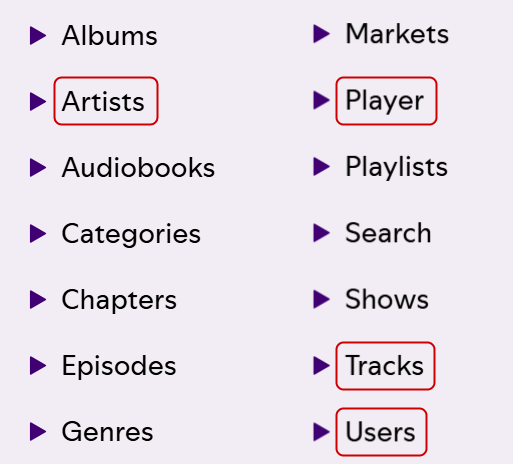
\includegraphics[width=0.4\textwidth]{figures/selected_groups.png}
    \caption{Grupos de endpoints ofrecidos y cuáles se van a usar.}
    \label{fig:selected_groups}
\end{figure}


\begin{figure}[H]
    \centering
    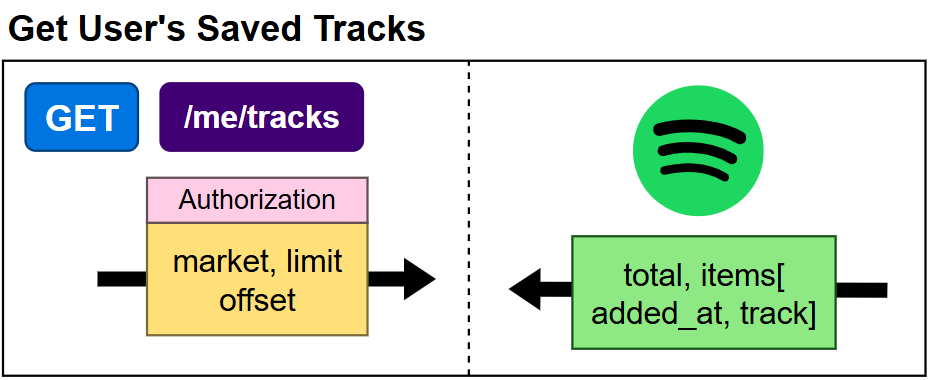
\includegraphics[width=\textwidth]{figures/endpoints/get_users_saved_tracks.png}
    \caption{Endpoint de \textit{Get User's Saved Tracks}.}
    \label{fig:get_usr_saved_tracks}
\end{figure}

\begin{figure}[H]
    \centering
    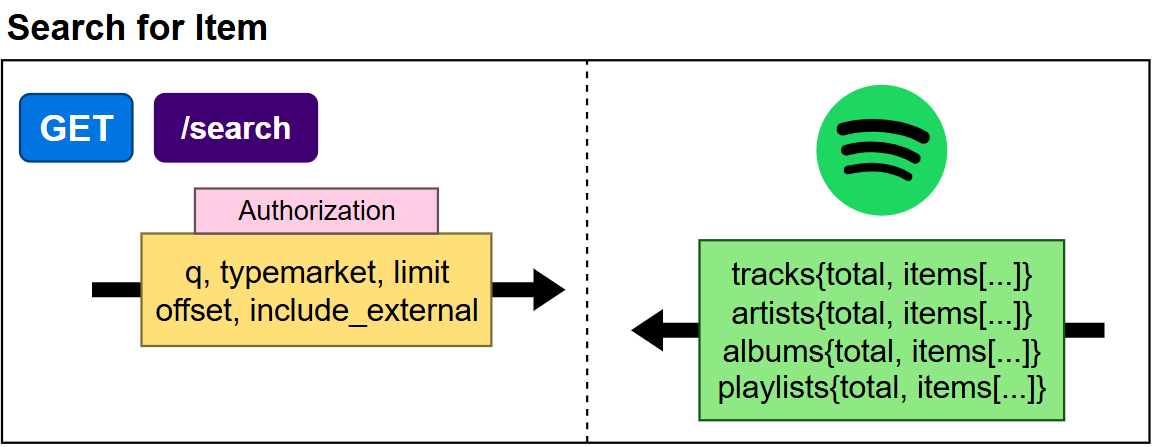
\includegraphics[width=\textwidth]{figures/endpoints/search_for_item.png}
    \caption{Endpoint de \textit{Search for Item}.}
    \label{fig:search_item}
\end{figure}

\begin{figure}[H]
    \centering
    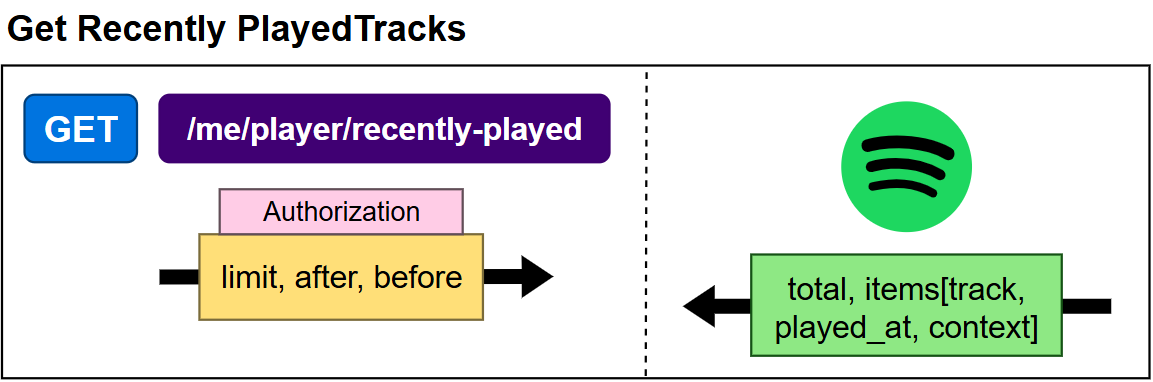
\includegraphics[width=\textwidth]{figures/endpoints/get_recently_played_tracks.png}
    \caption{Endpoint de \textit{Get Recently Played Tracks}.}
    \label{fig:get_recently_played_tracks}
\end{figure}

\begin{figure}[H]
    \centering
    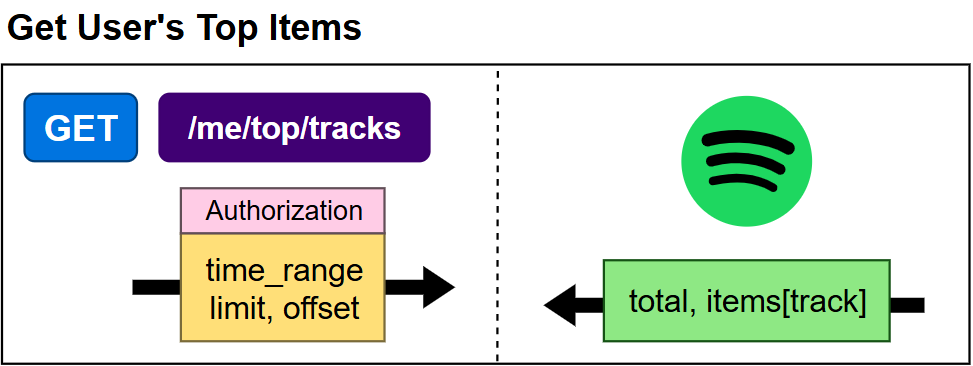
\includegraphics[width=\textwidth]{figures/endpoints/get_users_top_items.png}
    \caption{Endpoint de \textit{Get User's Top Items (Tracks)}.}
    \label{fig:get_usr_top_items_tracks}
\end{figure}

\begin{figure}[H]
    \centering
    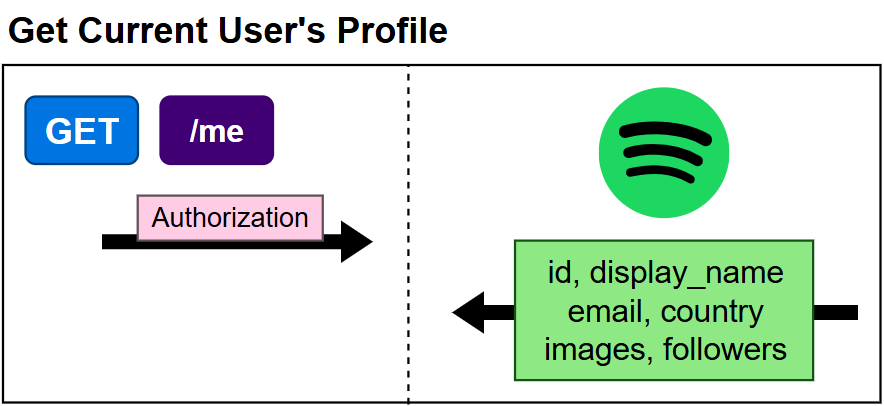
\includegraphics[width=\textwidth]{figures/endpoints/get_current_users_profile.png}
    \caption{Endpoint de \textit{Get Current User's Profile}.}
    \label{fig:get_current_usr_profile}
\end{figure}

\begin{figure}[H]
    \centering
    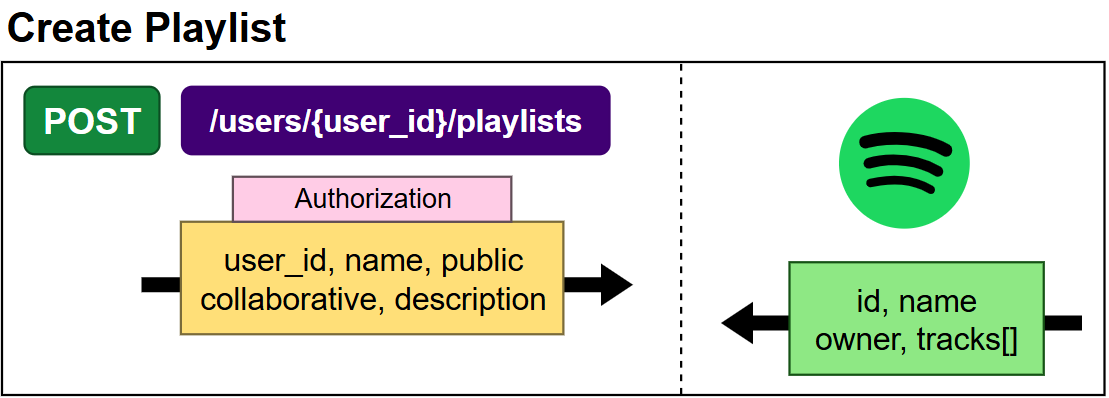
\includegraphics[width=\textwidth]{figures/endpoints/create_playlist.png}
    \caption{Endpoint de \textit{Create Playlist}.}
    \label{fig:create_playlist}
\end{figure}

\begin{figure}[H]
    \centering
    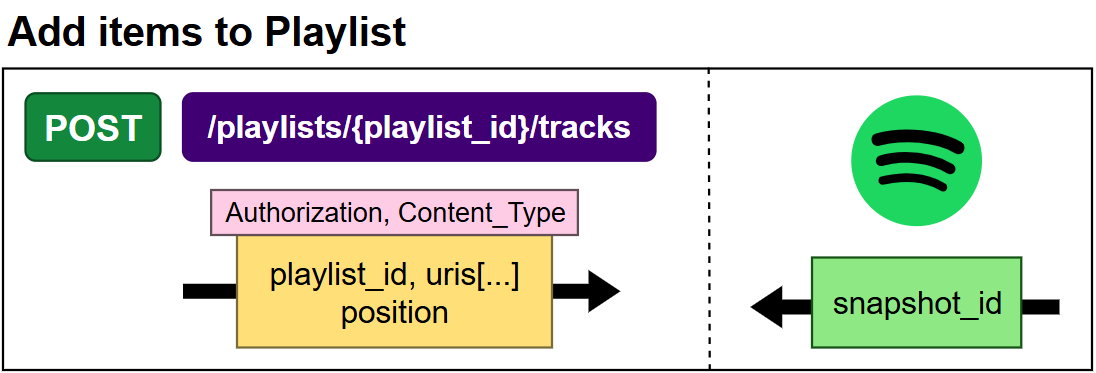
\includegraphics[width=\textwidth]{figures/endpoints/add_items_to_playlist.png}
    \caption{Endpoint de \textit{Add Items to Playlist}.}
    \label{fig:add_items_playlist}
\end{figure}

\begin{figure}[H]
    \centering
    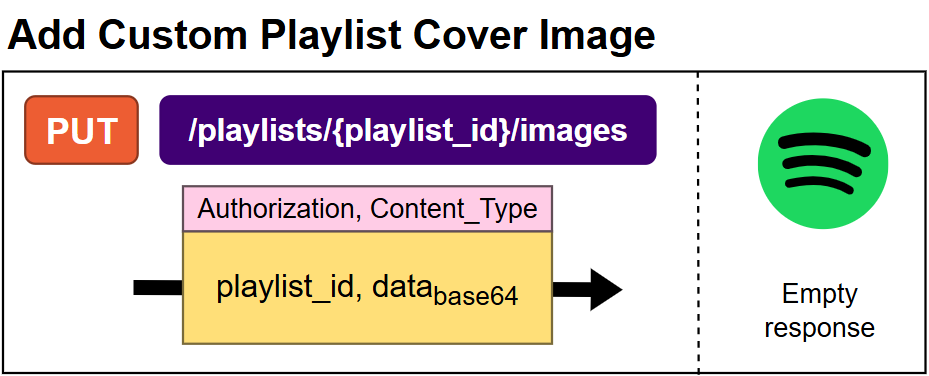
\includegraphics[width=\textwidth]{figures/endpoints/add_custom_playlist_cover_image.png}
    \caption{Endpoint de \textit{Add Custom Playlist Cover Image}.}
    \label{fig:add_custom_playlist_cover_img}
\end{figure}






\subsection{Limitaciones de la API}
\begin{itemize}
    \item \textbf{Restricciones técnicas}:
          \begin{itemize}
              \item Límite de peticiones por segundo/minuto (rate limit).
              \item Alcance limitado de datos (por ejemplo, máximo 50 resultados por llamada).
          \end{itemize}
    \item \textbf{Datos no disponibles}:
          \begin{itemize}
              \item Explicaría qué datos relevantes para mi proyecto no están accesibles (por ejemplo, datos de otros usuarios).
              \item Posibles soluciones, como procesar datos existentes para obtener métricas derivadas.
          \end{itemize}
    \item \textbf{Problemas de autenticación}: P.e., el tiempo limitado de vida del \texttt{access\_token}.
\end{itemize}

\subsection{Análisis de la Documentación Oficial}
\begin{itemize}
    \item Evaluaría la calidad de la documentación oficial, mencionando aspectos positivos y negativos:
          \begin{itemize}
              \item ¿Es fácil de entender?
              \item ¿Incluye ejemplos útiles?
              \item ¿Proporciona herramientas adicionales (como Spotify Console para probar peticiones)?
          \end{itemize}
    \item Relación con el soporte: ¿Existen foros, GitHub o recursos para resolver dudas?
\end{itemize}

\subsection{Ejemplos Prácticos y Flujo de Datos}
\begin{itemize}
    \item \textbf{Caso práctico 1}: Obtener las canciones más escuchadas y generar un gráfico.
          \begin{itemize}
              \item Explicaría cómo interactúan mi aplicación y la API:
                    \begin{itemize}
                        \item Envío del \texttt{access\_token}.
                        \item Recuperación de datos del endpoint \texttt{Get User's Top Tracks}.
                        \item Transformación de los datos en el frontend para visualizarlos.
                    \end{itemize}
          \end{itemize}
    \item \textbf{Caso práctico 2}: Usar el endpoint \texttt{Get Audio Features} para analizar las propiedades musicales de una canción.
          \begin{itemize}
              \item Incluiría un ejemplo de cómo combino diferentes endpoints para lograr una funcionalidad.
          \end{itemize}
\end{itemize}

\subsection{Soluciones Técnicas y Decisiones}
\begin{itemize}
    \item \textbf{Librerías usadas}: Si uso alguna librería para interactuar con la API (como Axios o Fetch en Next.js), lo mencionaría.
    \item \textbf{Procesamiento de datos}:
          \begin{itemize}
              \item Cómo almaceno datos temporales en el frontend o backend.
              \item Transformaciones realizadas en los datos antes de visualizarlos.
          \end{itemize}
    \item \textbf{Gestión de errores}: Cómo manejaré errores como:
          \begin{itemize}
              \item Token expirado (\texttt{401 Unauthorized}).
              \item Límite de peticiones alcanzado (\texttt{429 Too Many Requests}).
              \item Respuestas vacías.
          \end{itemize}
\end{itemize}

\subsection{Comparación con las Necesidades del Proyecto}
\begin{itemize}
    \item ¿Qué datos y funcionalidades cubre bien la API?
    \item ¿Qué datos tendré que procesar o calcular por mi cuenta?
    \item Justificación de las decisiones técnicas basadas en este análisis.
\end{itemize}

\subsection{Conclusión del Análisis}
\begin{itemize}
    \item Resumiría las capacidades clave de la API para mi proyecto.
    \item Identificaría los principales desafíos técnicos derivados de su uso.
    \item Explicaría cómo este análisis influirá en el diseño y la implementación del proyecto.
\end{itemize}




\section{Requisitos Funcionales}

\section{Requisitos No Funcionales}

\section{Casos de Uso}